\documentclass{article}
\usepackage[margin=1in]{geometry}
\usepackage{hyperref}
\usepackage[dvipsnames]{xcolor}
\usepackage{tikz}
\usepackage{subcaption}
\usepackage{amsmath, amsfonts}



\DeclareMathOperator{\Tr}{Tr}
\DeclareMathOperator{\diag}{\mathbf{diag}}
\DeclareMathOperator*{\argmin}{arg\,min}
\DeclareMathOperator*{\argmax}{arg\,max}

\newcommand{\E}{\mathbb{E}}
\newcommand{\bs}{\boldsymbol}

\newtheorem{theorem}{Theorem}
\newtheorem{lemma}[theorem]{Lemma}
\newtheorem{proposition}[theorem]{Proposition}
\newtheorem{claim}[theorem]{Claim}
\newtheorem{corollary}[theorem]{Corollary}
\newtheorem{definition}[theorem]{Definition}
\newenvironment{proof}{{\bf Proof:}}{\hfill\rule{2mm}{2mm}}


\title{On Farka's Lemma}
\author{
	Ruilin Li  \\
	\href{mailto:ruilin.li@gatech.edu}{ruilin.li@gatech.edu} \\
	Georgia Institute of Technology  
	}
\date{\today}

\begin{document}

\maketitle

\section{Farka's Lemma}
Farka's lemma (Farks's Alternative Theorem) is a useful tool and can be used to prove strong duality of linear programming and derive KKT condition with linear independence constraint qualification (LICQ).

\begin{lemma}[Farka's Lemma]
Given a vector $\bs{b} \in \mathbb{R}^m$  and $A \in \mathbb{R}^{m \times n}$, it must be one of the following two cases,
\begin{itemize}
	\item There exists a non-negative vector $\bs{x} \ge \bs{0}$ such that 
		\[ A\bs{x} = \bs{b} \]
	\item There exists a non-negativevector $\bs{y} \ge \bs{0}$ such that
		\[ A^T\bs{y} \le \bs{0} \mbox{ and } \bs{b}^T\bs{y} > 0 \]
\end{itemize}
See figure \ref{fig:farka} for visual illustration.
\end{lemma}

\begin{figure}[h]
\begin{subfigure}{.5\linewidth}
\centering
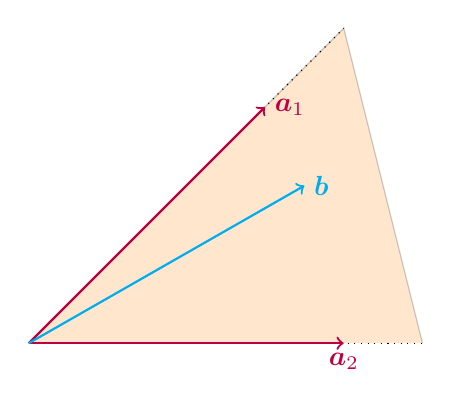
\begin{tikzpicture}
	\draw [fill=orange, opacity=0.2] (0,0) -- (4,4) -- (5,0);
	\draw [dotted] (0,0) -- (4,4);
	\draw [dotted] (0,0) -- (5,0);
	\draw [->, thick, purple] (0,0) -- (3,3);
	\node [right, purple] at (3,3) {$\bs{a}_1$};
	\draw [->, thick, purple] (0,0) -- (4,0);
	\node [below, purple] at (4,0) {$\bs{a}_2$};
	\draw [->, thick, cyan] (0,0) -- (3.5,2);
	\node [right, cyan] at (3.5,2) {$\bs{b}$};
\end{tikzpicture}
\caption{$A\bs{y} = \bs{b}$}\label{fig:case1}
\end{subfigure}
~
\begin{subfigure}{.5\linewidth}
\centering
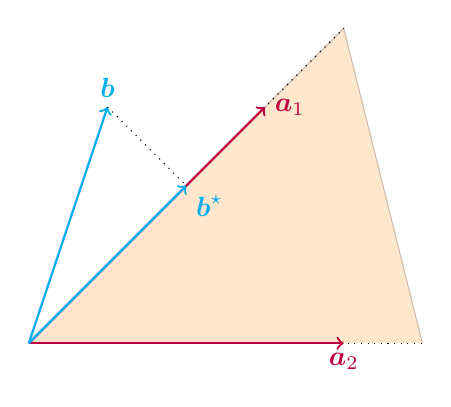
\begin{tikzpicture}
	\draw [fill=orange, opacity=0.2] (0,0) -- (4,4) -- (5,0);
	\draw [dotted] (0,0) -- (4,4);
	\draw [dotted] (0,0) -- (5,0);
	\draw [->, thick, purple] (0,0) -- (3,3);
	\node [right, purple] at (3,3) {$\bs{a}_1$};
	\draw [->, thick, purple] (0,0) -- (4,0);
	\node [below, purple] at (4,0) {$\bs{a}_2$};
	\draw [->, thick, cyan] (0,0) -- (1,3);
	\node [above, cyan] at (1,3) {$\bs{b}$};
	\draw [dotted] (1,3) -- (2,2);
	\draw [->, thick, cyan] (0,0) -- (2,2);
	\node [below right, cyan] at (2,2) {$\bs{b}^\star$};
\end{tikzpicture}
\caption{$A^T\bs{y} \le \bs{0} \mbox{ and } \bs{b}^T\bs{y} > 0$}\label{fig:case2}
\end{subfigure}
\caption{Visualization of Farka's Alternatives}\label{fig:farka}
\end{figure}

\begin{proof}
\begin{itemize}
	\item If there exists $\bs{x} \ge \bs{0}$ such that $A\bs{x}=\bs{b}$, then for any vector $\bs{y}$, we have 
	\[ \bs{y}^T\bs{b} = \bs{y}^T A\bs{x}=(A^T \bs{y})^T\bs{x} \]
	and it is impossible to find $\bs{y} \ge \bs{0}$ to satisfy $A^T \bs{y} \ge \bs{0}$ and $\bs{b}^T\bs{y} < 0$ at the same time.
	\item If there does not exist $\bs{x} \ge \bs{0}$ such that $A\bs{x} =\bs{b}$, denote the cone of formed by column vectors of $A$ by $C(A)$, 
	\[ C(A) = \{ \sum_{i=1}^m x_i \bs{a}_i| x_i \ge 0, i=1,2,\cdots, m\}\]
	Consider vector \[\bs{y} = \bs{b} - \bs{b}^\star\] where $\displaystyle \bs{b}^\star = \argmin_{\bs{x} \in C(A)} ||\bs{x} - \bs{b}||^2$.

	From the property of projection onto convex sets (POC), we have that for any vector $\bs{z} \in C(A)$,
	\[  \langle \bs{z} - \bs{b}^\star, \bs{b} - \bs{b}^\star \rangle \le 0, \quad \langle \bs{b} - \bs{b}^\star, \bs{b} - \bs{z}\rangle \ge 0\]
	and the second equality holds if and only if $\bs{b} =\bs{b}^\star$. By our assumption, $\bs{b} \notin C(A)$ so $\bs{b} \neq \bs{b}^\star$ hence $\langle \bs{b} - \bs{b}^\star, \bs{b} - \bs{z}\rangle > 0$. Let $\bs{z} =\bs{0}$, we immediate conclude that $\bs{b}^T\bs{y} > 0$.

	Next we would like to show $\langle \bs{z}, \bs{b} - \bs{b}^\star \rangle \le 0$ and it suffices to show $\langle \bs{b}^\star, \bs{b} - \bs{b}^\star\rangle =0$. This is due to the fact 
	\[ f(\alpha) = ||\alpha \bs{b}^\star - \bs{b}||^2 \]
	is minimized when $\alpha = 1$ and 
	\[f^\prime(1) = \langle \bs{b}^\star-\bs{b}, \bs{b}^\star \rangle = 0\]

	Therefore, we find a non-negative vector $\bs{y} \ge \bs{0}$ such that $A^T\bs{y} \ge \bs{0}$ and $\bs{y}^T\bs{b} > 0$.
\end{itemize}
\end{proof}



\end{document}